\documentclass[aspectratio=169]{beamer}
\usepackage{graphicx}
\usepackage[T1]{fontenc}
\usepackage{courier}
\usepackage{cite}
\usepackage[absolute,overlay]{textpos}
\usepackage[backend=biber]{biblatex}
\addbibresource{sources.bib}
%\usepackage[texcoord, grid,gridcolor=red!10,subgridcolor=green!10,gridunit=pt] {eso-pic}

\beamertemplatenavigationsymbolsempty
\setbeamertemplate{caption}[numbered]


%ref to this doc for future work: https://ctroupin.github.io/posts/2020-03-19-ppt2beamer/



%=============================================== COLOR CONFIGURATIONS
\definecolor{color1}{HTML}{003546}  %dark teal
\definecolor{color2}{HTML}{ffffff}  %white
\setbeamercolor{title}{fg=white}
\setbeamercolor{author}{fg=color2}
\setbeamercolor{institute}{fg=color2}
\setbeamercolor{frametitle}{fg=color1}
\setbeamercolor{date}{fg=color2}
\setbeamercolor{itemize item}{fg=color1}
\setbeamercolor{caption name}{fg=color1}


%=============================================== FOOT PAGE NUMBERS 
\setbeamertemplate{sidebar right}{}
\setbeamertemplate{footline}{%
\hfill\usebeamertemplate***{navigation symbols} 
\hspace{0.1cm} \vspace{0.1cm} \insertframenumber{} \hspace{0.2cm} \vspace{0.1cm}}


%----------------------- DOCUMENT BEGINS HERE.. ----------------------- %
\begin{document}


%=============================================== TITLE 

\begin{textblock*}{1000pt}(40pt,150pt)
\color{white}  \huge "SEO and Search Intent"
\end{textblock*}
\date{}


{ \usebackgroundtemplate{
\includegraphics[width=\paperwidth, height=\paperheight]{background1.pdf}}


\begin{textblock*}{1000pt}(45pt,200pt)
\color{white}  \small
 Timotej Mihálik 
\end{textblock*}

\maketitle
{\usebackgroundtemplate{
\includegraphics[width=\paperwidth]{background2.pdf}}

%=============================================== Rest of the slides

\begin{frame} {\huge Introduction}


\begin{itemize}
    \item<1-> What is SEO?
    \pause
    \item<2-> Different tipes of search Intents
    \pause
    \item<3-> How does search engine decide what sites to offer?
    \pause
    \item<4-> Manipulating search intent true optimization.
    \pause
    \item<5-> How to stay relevant for your customers.
    \pause
    \item<6-> Conclusion
    \pause
    \item<7-> Questions
\end{itemize}

\end{frame}

\begin{frame} {\huge What is SEO?}

\begin{itemize}
    \item<1-> SEO "Search Engine Optimization."
    \pause
    \item<2-> SEO falls under marketing fields.
    \pause
    \item<3-> It is the way how to get more sales or views on your domain.
    \pause
    
\end{itemize}
\end{frame}

\begin{frame} {\huge Different tips of search Intents}
\begin{itemize}
    \item<1-> What is search Intent?
    \pause
    \begin{itemize}
        \item<2-> Search intent is the thought behind a search.
        \pause
    \end{itemize}
    \item<3-> Search intent can be divided into four main categories:
    \pause
    \begin{itemize}
	\item<4-> 1.Informational Intent
 \pause
    \item<5-> 2.Navigational Intent
    \pause
    \item<6-> 3.Transactional Intent
    \pause
    \item<7-> 4.Commercial Investigation 
    \pause
 \end{itemize}
    \begin{figure}[]
        \visible<2>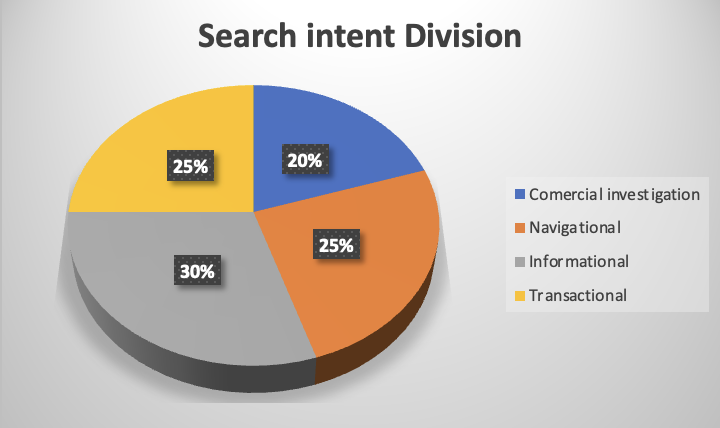
\includegraphics[width=0.4\textwidth]{pics/Pie graph 2.png} \caption{percentage distribution of Intents \cite{Picture1}} 
    \end{figure}
    
\end{itemize}
\end{frame}


\begin{frame} {\huge Search engine selection}
\begin{itemize}
    \item<1-> Steps of the selection 
    \begin{itemize}
        \item<2-> Algorithm and Bot sampling
        \item<3-> Universal algorithm 
        \item<4-> Fusion with users search history log 
        \end{itemize}
        \end{itemize}
    
\end{frame}

\begin{frame} {\huge Manipulation of SEO}
\begin{itemize}
    \item<1->Finding targeted audience
    \item<2-> Content Optimization for your audience 
        \begin{itemize}
            \item<3-> thru Use of key words
            \item<4-> Also using the right wording ex.("best apple")
        \end{itemize}
\end{itemize}

\end{frame} 
\begin{frame} {\huge  Staying relevant}
\begin{itemize}
    \item<1-> Try to appeal only to those who matter to you
    \item<2-> Be ware of misleading titles and texts 
    \item<3-> Don't force the user into nothing 
    \end{itemize}

\end{frame}

\begin{frame}{Conclusion}
\begin{figure}[]
        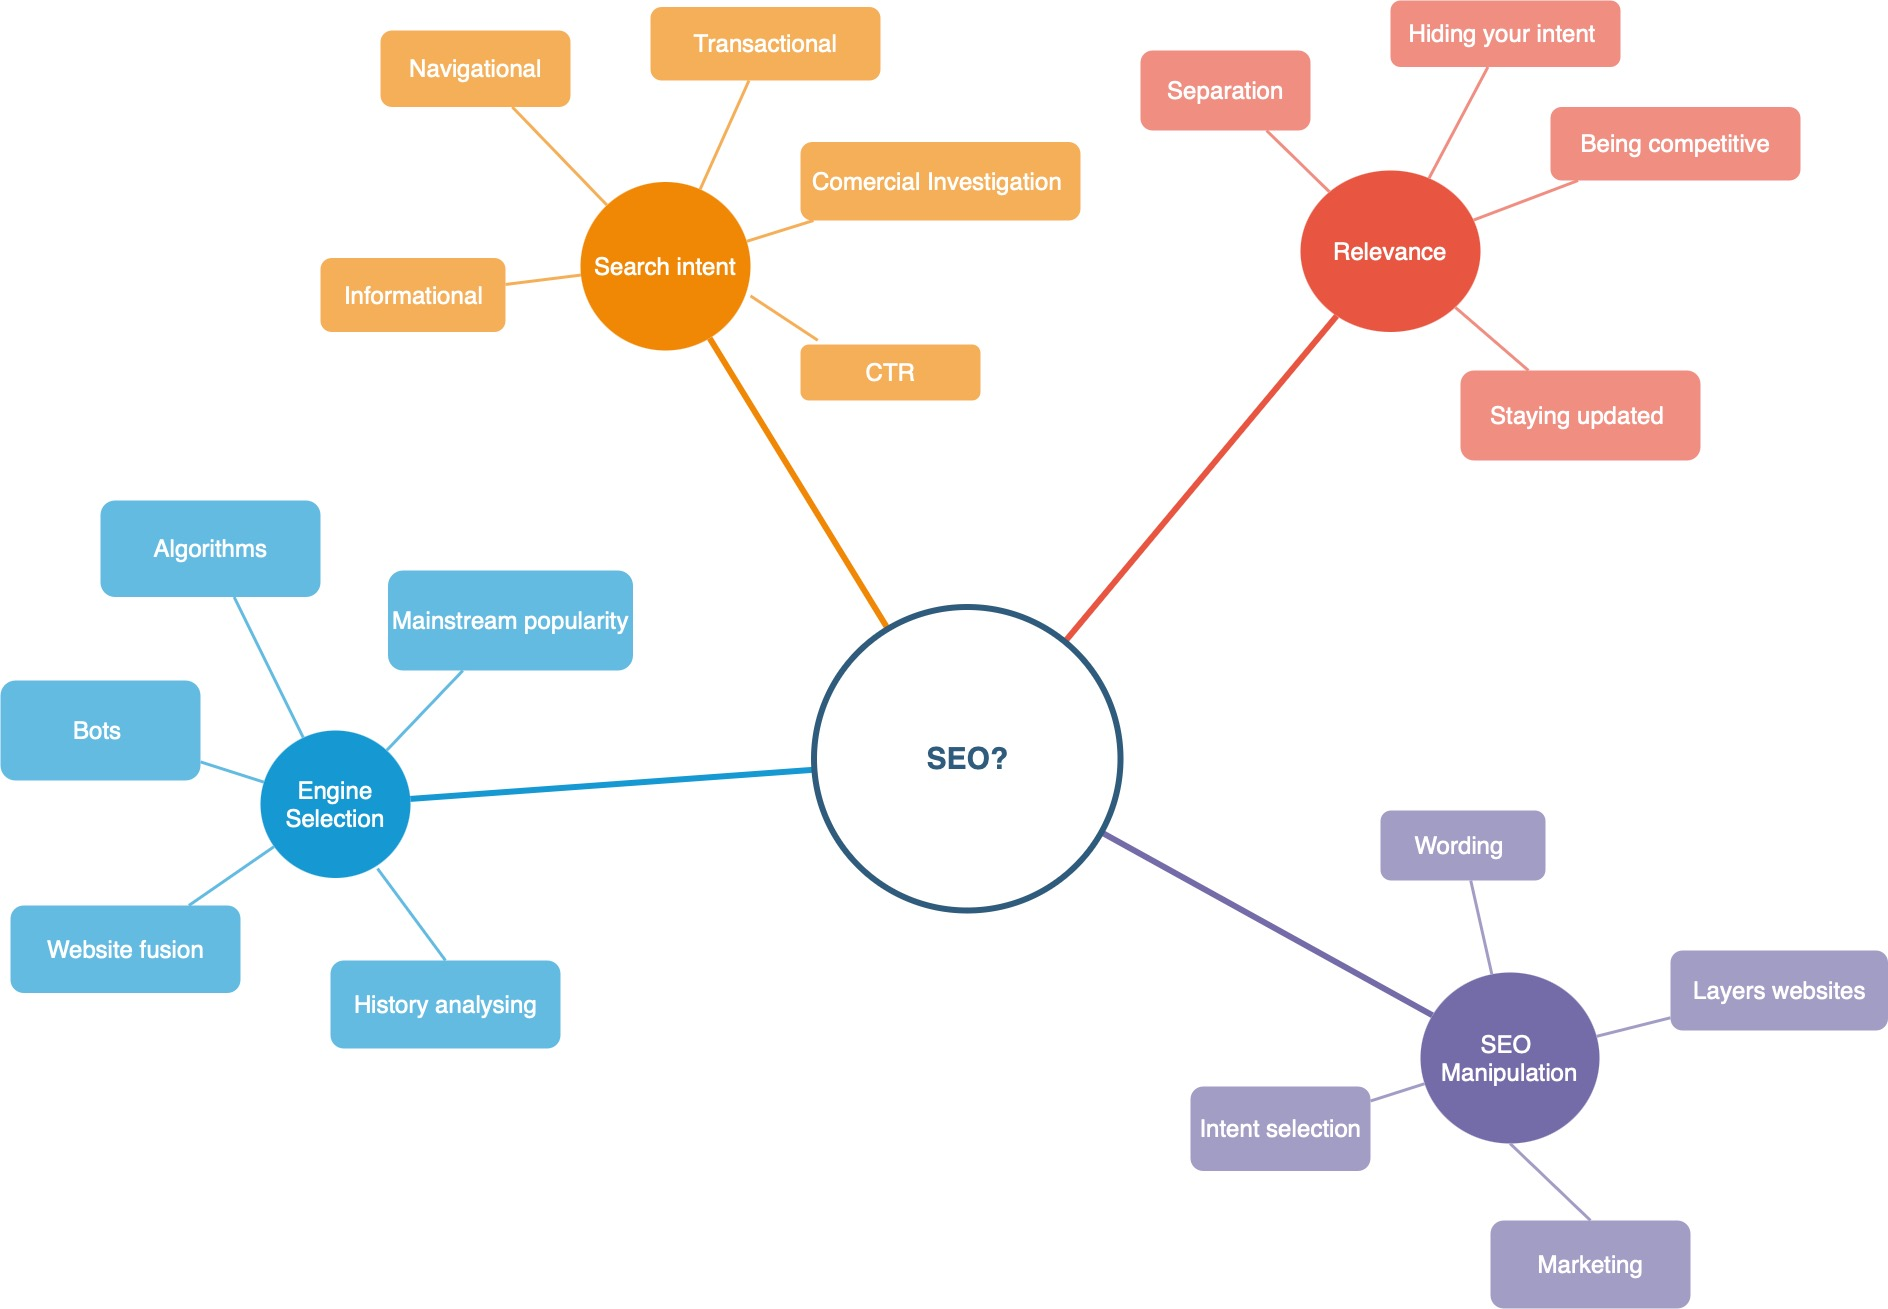
\includegraphics[width=0.7\textwidth]{pics/diagram 2.jpg} \caption{Conclusion scheme \cite{conclusion}} 
    \end{figure}
\end{frame}    


\begin{frame}{Sources}
\begin{itemize}
    \item Weizhu Chen Gang Wang Qiang Yang Botao Hu, Yuchen Zhang. Characte-
rizing search intent diversity into click models, 2011.
    \item Alexey Zagalsky Carlene Lebeuf, Margaret-Anne Storey. Software bots,
2018.
    \item Melius Weideman Eugene B. Visser. Fusing website usability and search
engine optimisation : original research, 2014.
    \item What is search intent and why is it important for SEO? Yoast, 2021.
    \item Xin Wu Jiarui Jin Youchen Fang Yong YU Jiarui Qin, Weinan Zhang. User
behavior retrieval for click-through rate prediction, 2020.
\item What Is SEO (Search Engine Optimization). Digitalspot academy, 2020.
\item Guorui zhou Xiaoqiang ZhU Kun Gai Qi PI, Weijie Bian. Practice on long
sequential user behavior modeling for click-through rate prediction, 2019
\item Gavin Turner. Content marketing, 2019.
    \end{itemize}
\end{frame}


\begin{frame}{Picture credits}
\printbibliography 
    
\end{frame}
\usebackgroundtemplate{
\includegraphics[width=\paperwidth]{background3.pdf}}
\begin{frame}
\color{white} \Huge Questions?
\end{frame} 
}


\AtEndDocument{
\usebackgroundtemplate{
\includegraphics[width=\paperwidth]{background3.pdf}}
\begin{frame}
\color{white} \Huge  "Thanks for the attention"
\end{frame} 
}


\end{document}
